% HEADER
\documentclass[class=article, crop=false]{standalone}
\usepackage{00_Preamble/frr_preamble}

% Packages
\usepackage{titlesec}
\usepackage{hyperref}
\usepackage{float}
\usepackage{graphics}
\usepackage{placeins}
\usepackage{adjustbox}
% END HEADER

\begin{document}
	\subsection{System Testing and Verification}
	\label{subsec:system_testing_and_verification}
	
	
	
	\subsubsection{Frame and Drive Testing}
	
	\begin{wrapfigure}{r}{0.35\textwidth}
		\centering
	 	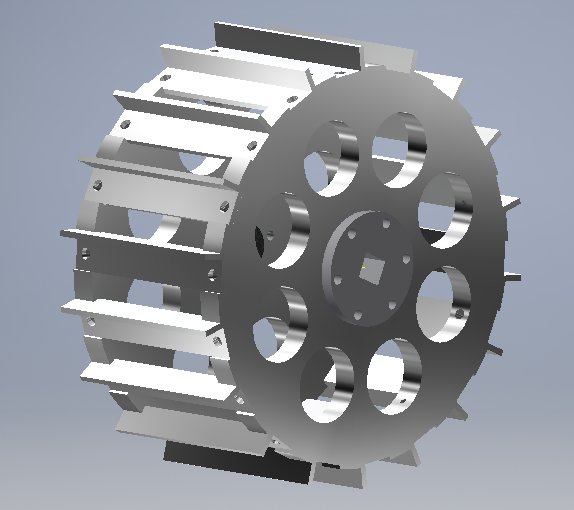
\includegraphics[width=0.30\textwidth]{09_Figures/final_wheel.png}
	 	\caption{CAD Model of Final Wheel Assembly}
	 	\label{fig:fan-cad}
	\end{wrapfigure}	
	
	The wheels must be tested for their performance in traversing the Martian terrain. It must be verified that there is not a lot of wheel slippage and that the autonomy sensors can accurately measure angular rotation. This, along with the optimal turning radius and the robot's ability to escape steep ditches, will be tested by driving the robot in a sandy environment. The environment will have obstacles similar in size to the ones on the RMC field, with sand and gravel representing the BP-1 and icy regolith, respectively.

The wheels were designed to be strong enough to carry the maximum allowed robot weight of 80 kg.  As a result, the wheels may be unnecessarily strong. The wheels' structural integrity will be tested in extreme conditions, where 50+ kg of gravel will be stored on the robot, so that the weight and power consumption can be reduced in future designs if possible.

	\subsubsection{Depositing System Testing}
	
	The depositing system must be tested to verify that it can store icy regolith, filter excess BP-1, and deposit icy regolith in the collection bin. This will be done by carrying out competition trial runs in a sandy environment. It will also be tested that the nylon mesh correctly filters BP-1 while retaining the icy regolith. A primary concern is that the filtered BP-1 will interfere with electrical components, as an electrical box containing most of the power distribution system rests directly under the conveyor. It will be verified that the electrical box was made dustproof by pouring dust onto the conveyor while the robot is running and confirming that all power systems remain active.
	Due to size constraints near the front of the frame, the conveyor had to be driven by a long roller chain at the back (Figure \ref{fig:conveyor_chain}). The chain may not have enough tension and the drive shaft could skip, which would cause the two roller chains that drive the conveyor to misalign. It must also be confirmed that icy regolith can be carried up the conveyor without sliding back down the incline. The nylon mesh will have a low coefficient of friction with the icy regolith, and small supports may need to be added to lift the icy regolith to the height of the collection bin. These factors will be tested by driving the conveyor under heavy icy regolith loads in competition trial runs.
		
	
	\FloatBarrier
		\begin{figure}[h]
			\centering
			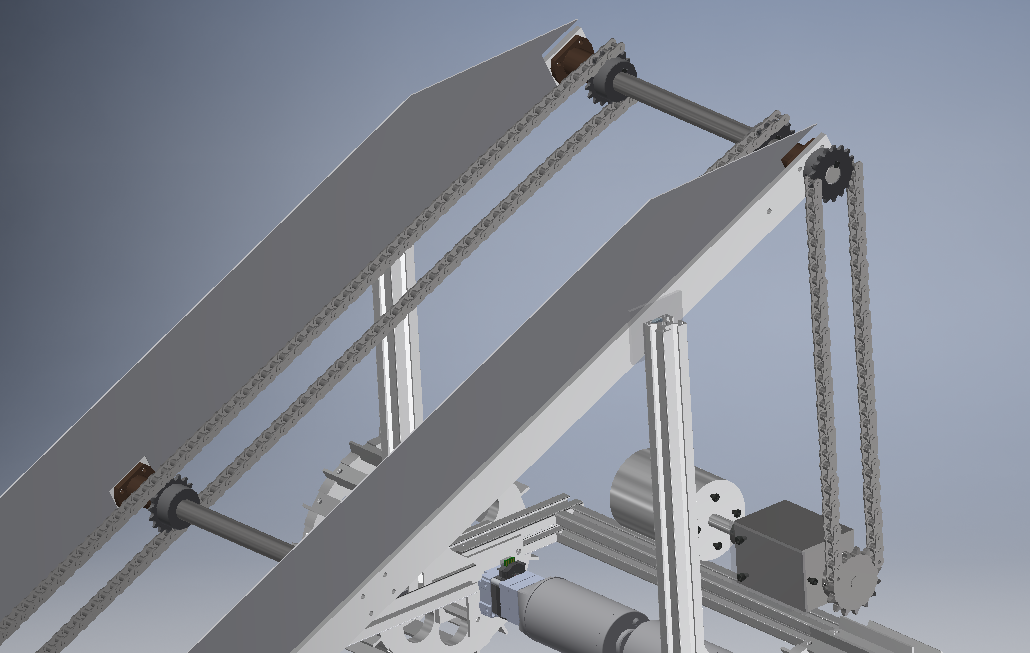
\includegraphics[width=0.5\linewidth]{09_Figures/conveyor_roller_chain.png}
			\caption{Conveyor Chain with Potential Tension Problems}
			\label{fig:conveyor_chain}
		\end{figure}
		\FloatBarrier
		
	
			
	
	

\end{document}
